\documentclass[
]{jss}

%% recommended packages
\usepackage{orcidlink,thumbpdf,lmodern}

\usepackage[utf8]{inputenc}

\author{
Piotr Chlebicki\\Stockholm University \And Maciej
Beręsewicz~\orcidlink{0000-0002-8281-4301}\\Poznań University of
Economics and Business\\
Statistical Office in Poznań
}
\title{\pkg{singleRcapture}: A Package for Single-Source
Capture-Recapture Models}

\Plainauthor{Piotr Chlebicki, Maciej Beręsewicz}
\Plaintitle{singleRcapture A Package for Single-Source Capture-Recapture
Models}
\Shorttitle{\pkg{singleRcapture}: Single-Source Capture-Recapture
Models}


\Abstract{
Estimating population size is an important issue in official statistics,
social sciences and natural sciences. One way to approach this problem
is to use capture-recapture methods, which can be classified according
to the number of sources used, the main distinction being between
methods based on one source and those based on two or more sources. In
this presentation we will introduce the \pkg{singleRcapture} R package
for fitting SSCR models. The package implements state-of-the-art models
as well as some new models proposed by the authors (e.g.~extensions of
zero-truncated one-inflated and one-inflated zero-truncated models). The
software is intended for users interested in estimating the size of
populations, particularly those that are difficult to reach or for which
information is available from only one source and dual/multiple system
estimation cannot be used.
}

\Keywords{population size estimation, hidden populations, truncated
distributuons, count regression models, \proglang{R}}
\Plainkeywords{population size estimation, hidden populations, truncated
distributuons, count regression models, R}

%% publication information
%% \Volume{50}
%% \Issue{9}
%% \Month{June}
%% \Year{2012}
%% \Submitdate{}
%% \Acceptdate{2012-06-04}

\Address{
    Piotr Chlebicki\\
    Stockholm University\\
    Matematiska institutionen\\
Albano hus 1\\
106 91 Stockholm, Sweden\\
  E-mail: \email{piotr.chlebicki@math.su.se}\\
  URL: \url{https://github.com/Kertoo},
\url{https://www.su.se/profiles/pich3772}\\~\\
      Maciej Beręsewicz\\
    Poznań University of Economics and Business\\
Statistical Office in Poznań\\
    Poznań University of Economics and Business\\
Department of Statistics\\
Institute of Informatics and Quantitative Economics\\
Al. Niepodległosci 10\\
61-875 Poznań, Poland\\
\strut \\
Statistical Office in Poznań\\
ul. Wojska Polskiego 27/29\\
60-624 Poznań, Poland\\
  E-mail: \email{maciej.beresewicz@ue.poznan.pl}\\
  
  }


% tightlist command for lists without linebreak
\providecommand{\tightlist}{%
  \setlength{\itemsep}{0pt}\setlength{\parskip}{0pt}}




\usepackage{amsmath, amsthm, amssymb} \usepackage{calc, ragged2e}

\DeclareMathAlphabet{\mathmybb}{U}{bbold}{m}{n}
\newcommand{\1}{\mathcal{I}} \newcommand{\bx}{\boldsymbol{x}}
\newcommand{\bX}{\boldsymbol{X}} \newcommand{\bbeta}{\boldsymbol{\beta}}
\newcommand{\boeta}{\boldsymbol{\eta}}

\begin{document}



\section{Introduction}\label{introduction}

Population size estimation is a\textasciitilde critical methodological
approach employed across multiple scientific disciplines, serving as
a\textasciitilde fundamental basis for research, policy formulation, and
decision-making processes. In the field of statistics, particularly
official statistics, precise population estimates are essential for
developing robust economic models, optimizing resource allocation, and
informing evidence-based policy formulation. Social scientists utilize
advanced population estimation techniques to investigate
\textit{hard-to-reach} populations, such as homeless individuals or
illicit drug users, thereby addressing the inherent limitations of
conventional census methodologies. These techniques are crucial for
obtaining accurate data on populations that are typically
under-represented or difficult to access through traditional sampling
methods. In ecology and epidemiology, researchers focus on estimating
the size of specific species or disease-affected populations within
defined geographical regions, which is vital for conservation efforts,
ecosystem management, and public health interventions.

Population size estimation can be approached through various
methodologies, each with distinct advantages and limitations.
Traditional approaches include full enumeration (e.g.~census operations)
and comprehensive sample surveys, which, while providing detailed data,
are often resource-intensive and may result in delayed estimates,
particularly for human populations. Alternative methods leverage
existing data sources, such as administrative registers or carefully
designed small-scale studies in wildlife research. A more sophisticated
approach, known as \textit{capture-recapture} or
\textit{multiple system estimation}, utilizes data from multiple
enumerations of the same population. This can be implemented using
a\textasciitilde single source with repeated observations, two distinct
sources, or multiple sources.

In this paper we focus specifically on methods that utilize
a\textasciitilde single data source with multiple enumerations of the
same units. In human population studies, such data might be derived from
police records, health system databases, or border control logs, while
for non-human populations, veterinary records or specialized field data
serve as analogous sources.

\subsection{How do we estimate population size with a single
register?}\label{how-do-we-estimate-population-size-with-a-single-register}

Let \(Y_{k}\) represent the number of times \(k\)-th unit was observed
in source data. Clearly, we don not know how often \(Y_{k}=0\) and to
find the total population size \(N\) we need to estimate it. In general,
we assume that conditional distribution of \(Y_{k}\) given
a\textasciitilde vector of covariates \(\boldsymbol{x}_{k}\) follows
some version of zero truncated count data distribution. Knowing the
parameters of the distribution we may estimate the population size using
Horwitz-Thompson type estimator: \begin{equation*}
    \hat{N}=
    \sum_{k=1}^{N}\frac{I_{k}}{\mathbb{P}[Y_{k}>0|\boldsymbol{X}_{k}]}=
    \sum_{k=1}^{N_{obs}}\frac{1}{\mathbb{P}[Y_{k}>0|\boldsymbol{X}_{k}]},
\end{equation*} where \(I_{k}:=\mathcal{I}_{\mathbb{N}}(Y_{k})\), and
maximum likelihood estimate of \(N\) is obtained after substituting
regression estimates for \(\mathbb{P}[Y_{k}>0|\boldsymbol{x}_{k}]\) into
the equation above. Most of the methods relate to poisson processes.

The analytic variance estimation is then done by computing two parts of
the decomposition due to the law of total variance:
\begin{equation}\label{law_of_total_variance_decomposition}
  \text{var}[\hat{N}]=
  \mathbb{E}\left[\text{var}
  \left[\hat{N}|I_{1},\dots,I_{n}\right]\right]+
  \text{var}\left[\mathbb{E}[\hat{N}|I_{1},\dots,I_{n}]\right],
\end{equation} where the first addend is by the multivariate \(\delta\)
method seen to be: \begin{equation}
  \mathbb{E}\left[\text{var}
  \left[\hat{N}|I_{1},\dots,I_{n}\right]\right]=
  \left.\left(\frac{\partial(N|I_1,\dots,I_N)}{\partial\boldsymbol{\beta}}\right)^{T}
  \text{cov}\left[\boldsymbol{\beta}\right]
  \left(\frac{\partial(N|I_1,\dots,I_N)}{\partial\boldsymbol{\beta}}\right)
  \right|_{\boldsymbol{\beta}=\hat{\boldsymbol{\beta}}},
\end{equation} while the later part of the decomposition in
\eqref{law_of_total_variance_decomposition} is under the assumption of
independence of \(I_{k}\)'s and after some omitted simplifications one
sees that this is optimally estimated via: \begin{align}
  \text{var}\left(\mathbb{E}(\hat{N}|I_{1},\dots,I_{n})\right)&=
  \text{var}\left(\sum_{k=1}^{N}\frac{I_{k}}{\mathbb{P}(Y_{k}>0)}\right)\nonumber\\
  &\approx\sum_{k=1}^{N_{obs}}\frac{1-\mathbb{P}(Y_{k}>0)}{\mathbb{P}(Y_{k}>0)^{2}},
\end{align} which forms the basis of confidence interval creation.
Confidence intervals are usually constructed under the assumption of
(asymptotic) normality of \(\hat{N}\) or asymptotic normality of
\(\ln(\hat{N}-N)\) (or log normality of \(\hat{N}\)). The latter of
which is an attempt to address a common criticism of student type
confidence intervals in SSCR, that is a possibly skewed distribution of
\(\hat{N}\), and results in the confidence interval of the form (for
confidence level of \(\alpha\)): \begin{equation*}
  \left(N_{obs}+\frac{\hat{N}-N_{obs}}{G},N_{obs}+\left(\hat{N}-N_{obs}\right)G\right),
\end{equation*} where: \begin{equation*}
  G = \exp\left(z\left(1-\frac{\alpha}{2}\right)
  \sqrt{\ln\left(1+\frac{\widehat{\text{Var}}(\hat{N})}{\left(\hat{N}-N_{obs}\right)^{2}}\right)}\right).
\end{equation*}

The estimator \(\hat{N}\) is best interpreted as being an estimator for
the total number of \underline{observable} units in the population since
we have no means of estimating the number of units in the population for
which the probability of being included in the data is \(0\)
cf.~\cite{ztpoisson}.

\subsection{Software for
capture-recapture}\label{software-for-capture-recapture}

The package is available on CRAN:
\url{CRAN.R-project.org/package=singleRcapture} while the extension is
available on:
\url{https://github.com/ncn-foreigners/singleRcaptureExtra}.

The \pkg{singleRcapture} package is an \proglang{R} language package
that focuses on implementing state of the art methods for frequentist
point and interval estimation of size of closed populations in
single-source capture-recapture (SSCR) setting (e.g.~estimation of the
population size of irregular migrants at set time point in a given
area).

The beginning of inference in single source capture-recapture dates back
to the seminal \cite{ztpoisson} paper in which the zero truncated
poisson model was applied to study the size of population of irregular
migrants in fours cities in Netherlands.

There are some packages implementing zero truncated count data models
such as \pkg{VGAM} and \pkg{countreg} and they can be integrated within
the \pkg{singleRcapture} ecosystem by the lightweight extention
\pkg{singleRcaptureExtra}.

\section{Basic usage}\label{basic-usage}

\subsection[The]{The \code{estimatePopsize}
function}\label{estimatePopsize-function}

The main function that \pkg{singleRcapture} is built around is
\code{estimatePopsize}. The leading design principle was to make using
\code{estimatePopsize} as close to standard \code{stats::glm} as
possible. The most important arguments are:

\begin{itemize}
    \item \code{formula} -- the main formula (i.e for the Poisson $\lambda$ parameter),
    \item \code{data} -- the \code{data.frame} (or \code{data.frame} coercible) object,
    \item \code{model} -- either a function a string or a family class object specifying which model should be used possible values are listed in documentation. The supplied argument should have the form \code{model =  "ztpoisson"}, \code{model = ztpoisson} or \code{model = ztpoisson(lambdaLink = "log")} the third way is the only one where the user may (but doesn't have to) select a link function.
    \item \code{method} -- numerical method used to fit regression \code{IRLS} or \code{optim},
    \item \code{popVar} -- a method for estimating variance of $\hat{N}$ and confidence interval creation (either bootstrap, analytic or skipping the estimation entirely),
    \item \code{controlMethod, controlModel, controlPopVar} -- control parameters for numerical fitting, specifying additional formulas (inflation, dispersion) and population size estimation respectively. We will tackle these arguments separately,
    \item \code{offset} -- a matrix of offset values with number of columns matching the number of distribution parameters providing offset values to each of linear predictors.
\end{itemize}

With the \code{formula, data, model} being the three arguments which
must be provided in \code{estimatePopsize} syntax.

\subsubsection[Example with R code]{Example with \proglang{R}
code}\label{r-code}

The package should be installed from CRAN
\url{https://cran.r-project.org/package=singleRcapture} with the usual
code:

\begin{CodeChunk}
\begin{CodeInput}
R> install.packages("singleRcapture")
\end{CodeInput}
\end{CodeChunk}

To showcase the main function let us recreate the zero truncated Poisson
model from \cite{ztpoisson} on the same data included in the package
under the name \code{netherlandsimmigrant}:

\begin{CodeChunk}
\begin{CodeInput}
R> library(singleRcapture)
R> head(netherlandsimmigrant)
\end{CodeInput}
\begin{CodeOutput}
  capture gender    age       reason       nation
1       1   male <40yrs Other reason North Africa
2       1   male <40yrs Other reason North Africa
3       1   male <40yrs Other reason North Africa
4       1   male <40yrs Other reason         Asia
5       1   male <40yrs Other reason         Asia
6       2   male <40yrs Other reason North Africa
\end{CodeOutput}
\end{CodeChunk}

This data set contains information about immigrants in four cities
(Amsterdam, Rotterdam, The Hague and Utrecht) in Netherlands that have
been staying in the country illegally in 1995 and have appeared in
police records that year. The number of times each individual appeared
in the records is included in the \code{capture} variable with the
available covariates being \code{gender, age, reason, nation} being
respectively the persons gender and age, reason for being captured and
region of the world from which each person comes:

\begin{CodeChunk}
\begin{CodeInput}
R> summary(netherlandsimmigrant)
\end{CodeInput}
\begin{CodeOutput}
    capture         gender         age                reason    
 Min.   :1.000   female: 398   <40yrs:1769   Illegal stay: 259  
 1st Qu.:1.000   male  :1482   >40yrs: 111   Other reason:1621  
 Median :1.000                                                  
 Mean   :1.162                                                  
 3rd Qu.:1.000                                                  
 Max.   :6.000                                                  
                    nation    
 American and Australia: 173  
 Asia                  : 284  
 North Africa          :1023  
 Rest of Africa        : 243  
 Surinam               :  64  
 Turkey                :  93  
\end{CodeOutput}
\end{CodeChunk}

The basic syntax is indeed vary similar to that of \code{glm} with the
output of the summary method being also quite simmilar except for the
additional results of the population size estimates:

\begin{CodeChunk}
\begin{CodeInput}
R> basicModel <- estimatePopsize(
+   formula = capture ~ gender + age + nation,
+   model   = ztpoisson(),
+   data    = netherlandsimmigrant
+ )
\end{CodeInput}
\begin{CodeOutput}
Warning in singleRcaptureinternalIRLSmultipar(dependent = y, covariates = X, :
Convergence at halfstepsize
\end{CodeOutput}
\begin{CodeInput}
R> summary(basicModel)
\end{CodeInput}
\begin{CodeOutput}

Call:
estimatePopsize.default(formula = capture ~ gender + age + nation, 
    data = netherlandsimmigrant, model = ztpoisson())

Pearson Residuals:
     Min.   1st Qu.    Median      Mean   3rd Qu.      Max. 
-0.486442 -0.486442 -0.298080  0.002093 -0.209444 13.910844 

Coefficients:
-----------------------
For linear predictors associated with: lambda 
                     Estimate Std. Error z value  P(>|z|)    
(Intercept)           -1.3411     0.2149  -6.241 4.35e-10 ***
gendermale             0.3972     0.1630   2.436 0.014832 *  
age>40yrs             -0.9746     0.4082  -2.387 0.016972 *  
nationAsia            -1.0926     0.3016  -3.622 0.000292 ***
nationNorth Africa     0.1900     0.1940   0.979 0.327398    
nationRest of Africa  -0.9106     0.3008  -3.027 0.002468 ** 
nationSurinam         -2.3364     1.0136  -2.305 0.021159 *  
nationTurkey          -1.6754     0.6028  -2.779 0.005445 ** 
---
Signif. codes:  0 '***' 0.001 '**' 0.01 '*' 0.05 '.' 0.1 ' ' 1

AIC: 1712.901
BIC: 1757.213
Residual deviance: 1128.553

Log-likelihood: -848.4504 on 1872 Degrees of freedom 
Number of iterations: 8
-----------------------
Population size estimation results: 
Point estimate 12690.35
Observed proportion: 14.8% (N obs = 1880)
Std. Error 2808.165
95% CI for the population size:
          lowerBound upperBound
normal      7186.449   18194.25
logNormal   8431.277   19718.31
95% CI for the share of observed population:
          lowerBound upperBound
normal     10.332933   26.16035
logNormal   9.534288   22.29793
\end{CodeOutput}
\end{CodeChunk}

One point which we should make while analysing this data set is that
there is a disproportionate number of individuals who were observed only
once (see table bellow):

\begin{CodeChunk}
\begin{CodeInput}
R> table(netherlandsimmigrant$capture)
\end{CodeInput}
\begin{CodeOutput}

   1    2    3    4    5    6 
1645  183   37   13    1    1 
\end{CodeOutput}
\end{CodeChunk}

Since there is a reasonable suspicion that the act of observing a unit
in the dataset may led to undesirable consequences from the point of
view of the subject of the observation (here possible deportation,
detainment or similar). For those reason one should

\begin{CodeChunk}
\begin{CodeInput}
R> set.seed(123456)
R> modelInflated <- estimatePopsize(
+     formula = capture ~ nation,
+     model   = oiztgeom(omegaLink = "cloglog"),
+     data    = netherlandsimmigrant,
+     controlModel = controlModel(
+         omegaFormula = ~ gender + age
+     ),
+     popVar = "bootstrap",
+     controlPopVar = controlPopVar(bootType = "semiparametric")
+ )
\end{CodeInput}
\begin{CodeOutput}
Warning in estimatePopsize.default(formula = capture ~ nation, model = oiztgeom(omegaLink = "cloglog"), : The (analytically computed) hessian of the score function is not negative define.
NOTE: Second derivative test failing does not 
        necessarily mean that the maximum of score function that was found 
        numericaly is invalid since R^k is not a bounded space.
Additionally in one inflated and hurdle models second derivative test often fails even on valid arguments.
\end{CodeOutput}
\begin{CodeOutput}
Warning in estimatePopsize.default(formula = capture ~ nation, model =
oiztgeom(omegaLink = "cloglog"), : Switching from observed information matrix
to Fisher information matrix because hessian of log-likelihood is not negative
define.
\end{CodeOutput}
\begin{CodeInput}
R> summary(modelInflated)
\end{CodeInput}
\begin{CodeOutput}

Call:
estimatePopsize.default(formula = capture ~ nation, data = netherlandsimmigrant, 
    model = oiztgeom(omegaLink = "cloglog"), popVar = "bootstrap", 
    controlModel = controlModel(omegaFormula = ~gender + age), 
    controlPopVar = controlPopVar(bootType = "semiparametric"))

Pearson Residuals:
    Min.  1st Qu.   Median     Mean  3rd Qu.     Max. 
-0.41643 -0.41643 -0.30127  0.00314 -0.18323 13.88376 

Coefficients:
-----------------------
For linear predictors associated with: lambda 
                     Estimate Std. Error z value  P(>|z|)    
(Intercept)           -1.2552     0.2149  -5.840 5.22e-09 ***
nationAsia            -0.8193     0.2544  -3.220  0.00128 ** 
nationNorth Africa     0.2057     0.1838   1.119  0.26309    
nationRest of Africa  -0.6692     0.2548  -2.627  0.00862 ** 
nationSurinam         -1.5205     0.6271  -2.425  0.01532 *  
nationTurkey          -1.1888     0.4343  -2.737  0.00619 ** 
-----------------------
For linear predictors associated with: omega 
            Estimate Std. Error z value  P(>|z|)    
(Intercept)  -1.4577     0.3884  -3.753 0.000175 ***
gendermale   -0.8738     0.3602  -2.426 0.015267 *  
age>40yrs     1.1745     0.5423   2.166 0.030326 *  
---
Signif. codes:  0 '***' 0.001 '**' 0.01 '*' 0.05 '.' 0.1 ' ' 1

AIC: 1677.125
BIC: 1726.976
Residual deviance: 941.5416

Log-likelihood: -829.5625 on 3751 Degrees of freedom 
Number of iterations: 10
-----------------------
Population size estimation results: 
Point estimate 6699.953
Observed proportion: 28.1% (N obs = 1880)
Boostrap sample skewness: 1.621389
0 skewness is expected for normally distributed variable
---
Bootstrap Std. Error 1719.353
95% CI for the population size:
lowerBound upperBound 
  5001.409  11415.969 
95% CI for the share of observed population:
lowerBound upperBound 
  16.46816   37.58941 
\end{CodeOutput}
\end{CodeChunk}

\subsubsection{Methods}\label{methods}

\begin{CodeChunk}
\begin{CodeInput}
R> (popEst <- popSizeEst(basicModel))
\end{CodeInput}
\begin{CodeOutput}
Point estimate: 12690.35
Variance: 7885790
95% confidence intervals:
          lowerBound upperBound
normal      7186.449   18194.25
logNormal   8431.277   19718.31
\end{CodeOutput}
\end{CodeChunk}

the \code{popEst} object is of the \code{popSizeEstResults} class and
\code{list} type and contains the following fields:

\begin{itemize}
  \item \code{pointEstimate}, \code{variance} -- numerics containing point estimate and variance of this estimate.
  \item \code{confidenceInterval} -- a \code{data.frame} with confidence intervals.
  \item \code{boot} -- If bootstrap was performed a numeric vector containing the $\hat{N}$ values from the bootstrap, 
  a character vector with value \code{"No bootstrap performed"} otherwise.
  \item \code{control} -- a \code{controlPopVar} object with controls used to obtained the object.
\end{itemize}

\small

\begin{CodeChunk}
\begin{CodeInput}
R> dfb <- dfbeta(basicModel)
R> apply(dfb, 2, quantile)
\end{CodeInput}
\begin{CodeOutput}
       (Intercept)    gendermale     age>40yrs    nationAsia nationNorth Africa
0%   -0.0099087522 -0.0905349870 -0.0200100686 -9.555875e-02      -9.660498e-02
25%  -0.0015325874 -0.0007770048  0.0001792918 -5.288544e-04      -8.417624e-04
50%   0.0001906118 -0.0002829978  0.0003789034  6.642632e-05      -1.768274e-04
75%   0.0005208531  0.0010171840  0.0006909682  1.199821e-04       8.674555e-05
100%  0.0866193889  0.0221346454  0.1600608767  1.799137e-01       3.125955e-02
     nationRest of Africa nationSurinam  nationTurkey
0%          -9.449682e-02 -9.313832e-02 -9.619821e-02
25%         -2.436010e-04 -6.484354e-05 -2.199798e-04
50%          2.984337e-05  2.101820e-05  7.918083e-05
75%          8.278833e-05  3.676223e-05  1.427685e-04
100%         1.097872e-01  9.933828e-01  3.209798e-01
\end{CodeOutput}
\end{CodeChunk}

\normalsize

\begin{CodeChunk}
\begin{CodeInput}
R> dfp <- dfpopsize(basicModel, dfbeta = dfb)
R> summary(dfp)
\end{CodeInput}
\begin{CodeOutput}
     Min.   1st Qu.    Median      Mean   3rd Qu.      Max. 
-4236.407     2.660     2.660     5.445    17.281   117.445 
\end{CodeOutput}
\end{CodeChunk}

\subsection{Marginal frequencies}\label{marginal-frequencies}

A popular method of testing the model fit in single source
capture-recapture studies is comparing the fitted marginal frequencies
\(\displaystyle\sum_{j=1}^{N_{obs}}\hat{\mathbb{P}}\left[Y_{j}=k|\boldsymbol{x}_{j}, Y_{j} > 0\right]\)
with the observed marginal frequencies
\(\displaystyle\sum_{j=1}^{N}\mathcal{I}_{\{k\}}(Y_{k})=\sum_{j=1}^{N_{obs}}\mathcal{I}_{\{k\}}(Y_{k})\)
for \(k\geq1\). If a fitted model bears sufficient resemblance to the
real data collection process these quantities should be quite close and
both \(G\) and \(\chi^{2}\) tests may be employed in order to test the
statistical significance of the discrepancy with the following
\pkg{singleRcapture} syntax:

\begin{CodeChunk}
\begin{CodeInput}
R> margFreq <- marginalFreq(basicModel)
R> summary(margFreq, df = 1, dropl5 = "group")
\end{CodeInput}
\begin{CodeOutput}
Test for Goodness of fit of a regression model:

                 Test statistics df P(>X^2)
Chi-squared test           50.06  1 1.5e-12
G-test                     34.31  1 4.7e-09

-------------------------------------------------------------- 
Cells with fitted frequencies of < 5 have been grouped 
Names of cells used in calculating test(s) statistic: 1 2 3  
\end{CodeOutput}
\end{CodeChunk}

where the \code{dropl5} argument is used to indicate how to handle the
cells with less than \(5\) fitted observations, note however that
currently there is no continuity correction.

\subsection{Plots}\label{plots}

The \code{singleRStaticCountData} class has a \code{plot} method
implementing several types of quick demonstrative plots such as the
rootogram \cite{rootogram} for comparing the fitted and marginal
frequencies which we can get with the syntax:

\begin{CodeChunk}
\begin{CodeInput}
R> plot(basicModel, plotType = "rootogram")
\end{CodeInput}


\begin{center}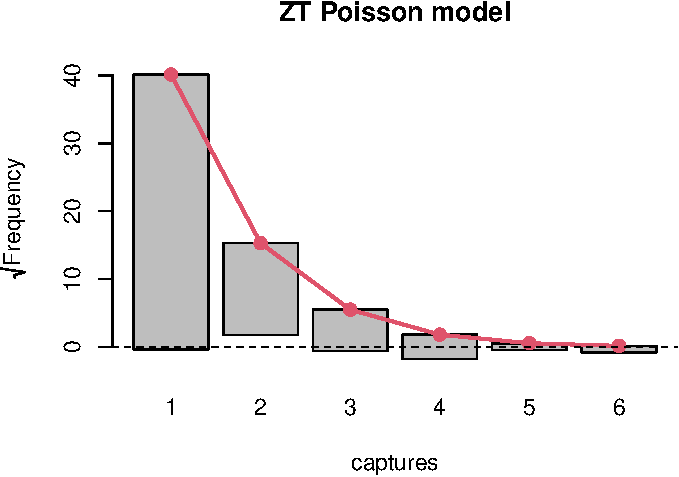
\includegraphics{singleRcapture_files/figure-latex/rootogram-1} \end{center}

\end{CodeChunk}

The comparison of deletion effect on population size estimate and
inverse probability weights:

\begin{CodeChunk}
\begin{CodeInput}
R> plot(basicModel, plotType = "dfpopContr", dfpop = dfp)
\end{CodeInput}


\begin{center}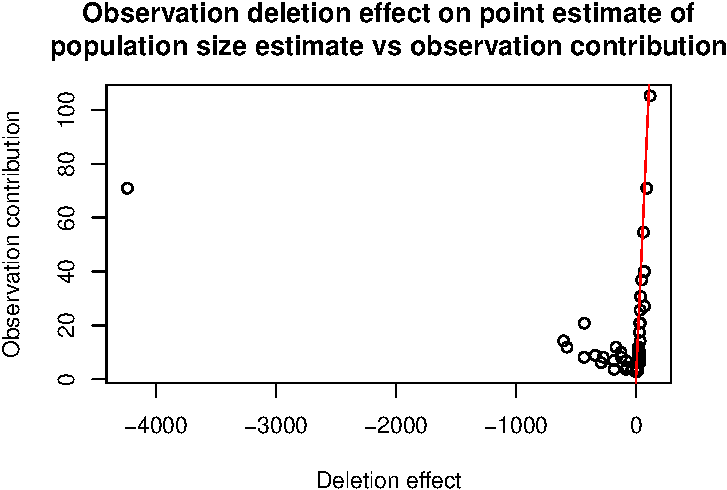
\includegraphics{singleRcapture_files/figure-latex/dfpopsize_plot-1} \end{center}

\end{CodeChunk}

and the plot that showcases stratisfied stimates:

\begin{CodeChunk}
\begin{CodeInput}
R> par(mar = c(2.5, 8.5, 4.1, 2.5), cex.main = .7, cex.lab = .6)
R> plot(basicModel, plotType = "strata")
\end{CodeInput}


\begin{center}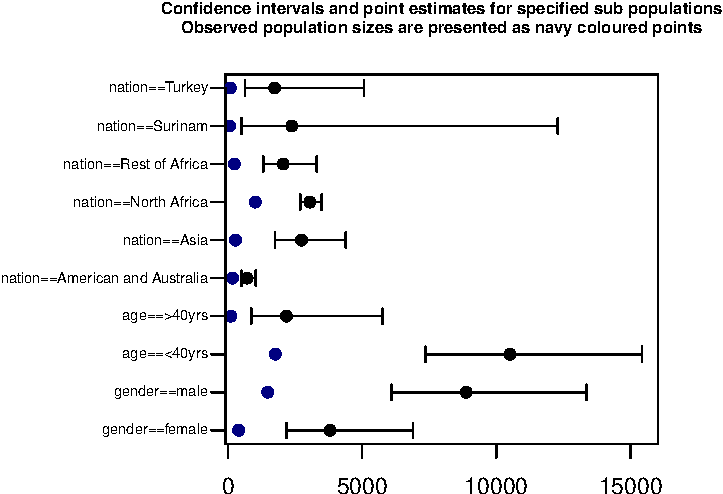
\includegraphics{singleRcapture_files/figure-latex/strata_plot-1} \end{center}

\end{CodeChunk}

the information which was supplied to the plot function above comes from
the \code{stratifyPopsize} method: \small

\begin{CodeChunk}
\begin{CodeInput}
R> stratifyPopsize(basicModel)
\end{CodeInput}
\begin{CodeOutput}
   Observed  Estimated ObservedPercentage  StdError normalLowerBound
1       398  3811.0911          10.443203 1153.9733       1549.34513
2      1482  8879.2594          16.690581 1812.0790       5327.64991
3      1769 10506.8971          16.836560 2017.2284       6553.20200
4       111  2183.4535           5.083690 1132.4502        -36.10819
5       173   708.3688          24.422308  132.8183        448.04969
6       284  2742.3147          10.356215  655.0929       1458.35623
7      1023  3055.2033          33.483860  201.2387       2660.78263
8       243  2058.1533          11.806701  493.2612       1091.37903
9        64  2386.4513           2.681806 2380.1835      -2278.62266
10       93  1739.8592           5.345260 1008.1794       -236.13602
   normalUpperBound logNormalLowerBound logNormalUpperBound
1         6072.8372           2189.0443            6902.133
2        12430.8689           6090.7762           13354.880
3        14460.5922           7359.4155           15426.455
4         4403.0151            872.0130            5754.876
5          968.6878            504.6086            1037.331
6         4026.2732           1755.2548            4391.590
7         3449.6240           2697.4900            3489.333
8         3024.9276           1318.7466            3305.786
9         7051.5252            505.2457           12287.983
10        3715.8544            638.0497            5068.959
                             name confLevel
1                  gender==female      0.05
2                    gender==male      0.05
3                     age==<40yrs      0.05
4                     age==>40yrs      0.05
5  nation==American and Australia      0.05
6                    nation==Asia      0.05
7            nation==North Africa      0.05
8          nation==Rest of Africa      0.05
9                 nation==Surinam      0.05
10                 nation==Turkey      0.05
\end{CodeOutput}
\end{CodeChunk}

\normalsize

The full list of plot types along with the list of optional arguments
which may be passed from the call to the \code{plot} method down to base
\proglang{R} and \pkg{graphics} functions is listed in the help file:

\begin{CodeChunk}
\begin{CodeInput}
R> ?plot.singleRStaticCountData
\end{CodeInput}
\end{CodeChunk}

\subsubsection[The stratifyPopsize method]{The \code{stratifyPopsize}
method}\label{the-method}

As previously showcased the \code{stratifyPopsize} may be used to
estimate the population sizes for different stratas using the same
fitted regression model as previously computed using the call to the
\code{estimatePopsize} function. The method for
\code{singleRStaticCountData} class accepts three optional parameters
\code{stratas, alpha, cov} which correspond to specification of sub
populations, the significance levels and the covariance matrix that will
be used to compute standard errors.

The full call is of the type: \footnotesize

\begin{CodeChunk}
\begin{CodeInput}
R> library(sandwich)
\end{CodeInput}
\begin{CodeOutput}
Warning: package 'sandwich' was built under R version 4.3.3
\end{CodeOutput}
\begin{CodeInput}
R> stratifyPopsize(
+   object  = basicModel,
+   stratas = ~ gender / (nation + age), 
+   alpha   = rep(c(.1, .2, .3, .4, .5), 
+                 length.out = 18),
+   cov     = vcovHC(basicModel, type = "HC4")
+ )
\end{CodeInput}
\begin{CodeOutput}
   Observed Estimated ObservedPercentage   StdError normalLowerBound
1       398 3811.0911          10.443203 1282.09956       1702.22504
2      1482 8879.2594          16.690581 1999.39209       6316.93533
3        67  328.8780          20.372297   84.81957        240.96814
4       106  379.4908          27.932167   83.91530        308.86588
5        62  775.9054           7.990665  303.01257        571.52651
6       222 1966.4093          11.289613  603.18021        974.26616
7       169  644.0545          26.240014  116.46407        494.79982
8       854 2411.1488          35.418801  172.33202       2232.53812
9        65  682.1776           9.528310  218.28791        498.46186
10      178 1375.9757          12.936275  369.03697       1127.06403
11       20  931.4677           2.147149  985.54139       -689.60358
12       44 1454.9835           3.024089 1520.27163       -493.32295
13       15  448.6079           3.343677  300.30767        137.35901
14       78 1291.2513           6.040652  733.06058        674.29194
15      378 3169.8263          11.924944  937.42614       2537.54198
16     1391 7337.0708          18.958520 1313.47160       5176.60226
17       20  641.2648           3.118836  453.82492         59.66481
18       91 1542.1886           5.900705  887.97851        621.85804
   normalUpperBound logNormalLowerBound logNormalUpperBound
1         5919.9573           2275.6416           6602.1612
2        11441.5835           6745.5675          11877.8858
3          416.7878            255.7692            430.3013
4          450.1157            318.4739            458.0301
5          980.2842            604.5269           1001.4205
6         2958.5525           1225.6476           3253.9046
7          793.3092            517.5628            816.4495
8         2589.7594           2242.8856           2599.7970
9          865.8933            527.2996            888.9423
10        1624.8873           1155.7975           1645.7331
11        2552.5391            234.3583           3895.6296
12        3403.2900            502.1052           4389.8894
13         759.8568            241.6446            844.5624
14        1908.2106            836.6593           2018.2367
15        3802.1106           2617.4717           3858.4164
16        9497.5393           5543.4798           9905.3720
17        1222.8649            288.7316           1456.2658
18        2462.5192            899.8794           2694.5381
                                        name confLevel
1                             gender==female       0.1
2                               gender==male       0.2
3  genderfemale:nationAmerican and Australia       0.3
4    gendermale:nationAmerican and Australia       0.4
5                    genderfemale:nationAsia       0.5
6                      gendermale:nationAsia       0.1
7            genderfemale:nationNorth Africa       0.2
8              gendermale:nationNorth Africa       0.3
9          genderfemale:nationRest of Africa       0.4
10           gendermale:nationRest of Africa       0.5
11                genderfemale:nationSurinam       0.1
12                  gendermale:nationSurinam       0.2
13                 genderfemale:nationTurkey       0.3
14                   gendermale:nationTurkey       0.4
15                    genderfemale:age<40yrs       0.5
16                      gendermale:age<40yrs       0.1
17                    genderfemale:age>40yrs       0.2
18                      gendermale:age>40yrs       0.3
\end{CodeOutput}
\end{CodeChunk}

\normalsize

where we used the \code{vcovHC} method for \code{singleRStaticCountData}
class from the \pkg{sandwitch} package, different significance levels
for confidence intervals in each strata and a formula to specify that we
wanted estimates for both males and females subdivided by \code{nation}
and \code{age}. The \code{stratas} parameter may be specified either as:

\begin{itemize}
\item a formula with empty left hand side which we have seen here,
\item a logical vector with number of entries equal to number of rows in the dataset in which case only one strata will be created,
\item a (named) list where each element is a logical vector, names of the list will be used to specify names variable in returned object,
\item a vector of names of explanatory variables which will result in every level of explanatory variable having its own sub population for each variable specified,
\item or not supplied at all in which case stratas will correspond to levels of each factor in the data without any interactions (string vectors will be converted to factors for the convenience of the user).
\end{itemize}

For plotting only the \code{logNormal} type of confidence interval is
used since the studentized confidence intervals often result in negative
lower bounds.

\section{Detailed information}\label{detailed-information}

\subsection{Fitting method}\label{fitting-method}

As previously showcased the \pkg{singleRcapture} package supports
modelling (linear) dependence on covariates of all parameters. To that
end a modified IRLS algorithm is employed, full details are available in
\cite{VGAM-main}. In order to employ the algorithm a modified model
matrix is created \(\boldsymbol{X}_{\text{vlm}}\) at call to
\code{estimatePopsize}. In the context of the models implemented in
\pkg{singleRcapture} this matrix can be written as:
\begin{equation}\label{X_vlm-definition}
  \boldsymbol{X}_{vlm}=
  \begin{pmatrix}
    \boldsymbol{X}_{1} & \boldsymbol{0} &\dotso &\boldsymbol{0}\cr
    \boldsymbol{0} & \boldsymbol{X}_{2} &\dotso &\boldsymbol{0}\cr
    \vdots & \vdots & \ddots & \vdots\cr
    \boldsymbol{0} & \boldsymbol{0} &\dotso &\boldsymbol{X}_{p}
  \end{pmatrix}
\end{equation} where each \(\boldsymbol{X}_{i}\) corresponds to a model
matrix associated with user specified formula.

In the context of multi-parameter families we have a matrix of linear
predictors \(\boldsymbol{\eta}\) instead of a vector, with the number of
columns matching the number of parameters in the distribution.
``Weights'' are then modified to be information matrices
\(\displaystyle\mathbb{E}\left[-\frac{\partial^{2}\ell}{\partial\boldsymbol{\eta}_{(k)}^{T}\partial\boldsymbol{\eta}_{(k)}}\right]\)
where \(\boldsymbol{\eta}_{(k)}\) is the \(k\)'th row of
\(\boldsymbol{\eta}\), while in the usual IRLS they are scalars
\(\displaystyle\mathbb{E}\left[-\frac{\partial^{2}\ell}{\partial\eta_{k}^{2}}\right]\)
which is often just
\(\displaystyle-\frac{\partial^{2}\ell}{\partial\eta^{2}}\).

\begin{enumerate}
    \justifying
    \item Initialize with \code{iter}$\leftarrow 1, \boldsymbol{\eta}\leftarrow$\code{start}
    $, \boldsymbol{W}\leftarrow I, \ell\leftarrow\ell(\boldsymbol{\beta})$.
    \item Store values from the previous step: 
    $\ell_{-}\leftarrow\ell, \boldsymbol{W}_{-}\leftarrow\boldsymbol{W}, \boldsymbol{\beta}_{-}\leftarrow\boldsymbol{\beta}$ 
    (the last assignment is omitted during the first iteration), and assign values in current iteration 
    $\displaystyle\boldsymbol{\eta}\leftarrow\boldsymbol{X}_{\text{vlm}}\boldsymbol{\beta}+\boldsymbol{o}, \boldsymbol{W}_{(k)}\leftarrow\mathbb{E}\left[-\frac{\partial^{2}\ell}{\partial\boldsymbol{\eta}_{(k)}^{T}\partial\boldsymbol{\eta}_{(k)}}\right], Z\leftarrow\boldsymbol{\eta}_{(k)}+\frac{\partial\ell}{\partial\boldsymbol{\eta}_{(k)}}\boldsymbol{W}_{(k)}^{-1}-\boldsymbol{o}_{(k)}$.
    \item Assign current coefficient value: 
    $\boldsymbol{\beta}\leftarrow\left(\boldsymbol{X}_{\text{vlm}}\boldsymbol{W}\boldsymbol{X}_{\text{vlm}}\right)^{-1}\boldsymbol{X}_{\text{vlm}}\boldsymbol{W}\boldsymbol{Z}$.
    \item If $\ell(\boldsymbol{\beta})<\ell(\boldsymbol{\beta}_{-})$ try selecting the smallest value $h$ such that for
    $\boldsymbol{\beta}_{h}\leftarrow2^{-h}\left(\boldsymbol{\beta}+\boldsymbol{\beta}_{-}\right)$ the inequality $\ell(\boldsymbol{\beta}_{h})>\ell(\boldsymbol{\beta}_{-})$ 
    holds if this is successful $\boldsymbol{\beta}\leftarrow\boldsymbol{\beta}_{h}$ else stop the algorithm.
    \item If convergence is achieved or \code{iter} is higher than \code{maxiter} end algorithm, 
    else \code{iter}$\leftarrow 1+$\code{iter} and return to step 2.
\end{enumerate}

\subsection[The]{The \code{estimatePopsizeFit}
function}\label{estimatePopsizeFit-function}

\begin{CodeChunk}
\begin{CodeInput}
R> X <- matrix(data = 0, nrow = 2 * NROW(farmsubmission), ncol = 7)
R> X[1:NROW(farmsubmission), 1:4] <- model.matrix(
+ ~ 1 + log_size + log_distance + C_TYPE, 
+ farmsubmission
+ )
R> X[-(1:NROW(farmsubmission)), 5:7] <- X[1:NROW(farmsubmission), c(1, 3, 4)]
R> # this attribute tells the function which elements of the design matrix 
R> # correspond to which linear predictor 
R> attr(X, "hwm") <- c(4, 3)
R> start <- glm.fit(# get starting points
+   y = farmsubmission$TOTAL_SUB, 
+   x = X[1:NROW(farmsubmission), 1:4], 
+   family = poisson()
+ )$coefficients
R> res <- estimatePopsizeFit(
+   y            = farmsubmission$TOTAL_SUB, 
+   X            = X, 
+   method       = "IRLS", 
+   priorWeights = 1, 
+   family       = ztoigeom(), 
+   control      = controlMethod(silent = TRUE), 
+   coefStart    = c(start, 0, 0, 0),
+   etaStart     = matrix(X %*% c(start, 0, 0, 0), ncol = 2),
+   offset       = cbind(rep(0, NROW(farmsubmission)), 
+                        rep(0, NROW(farmsubmission)))
+ )# extract results
R> ll <- ztoigeom()$makeMinusLogLike(y = farmsubmission$TOTAL_SUB, X = X)
R> print(c(res$beta, -ll(res$beta), res$iter))
\end{CodeInput}
\begin{CodeOutput}
[1] -2.784523e+00  6.170270e-01 -6.455925e-02  5.346108e-01 -3.174491e+00
[6]  1.280589e-01 -1.086452e+00 -1.727876e+04  1.500000e+01
\end{CodeOutput}
\begin{CodeInput}
R> # Compare with optim call
R> res2 <- estimatePopsizeFit(
+   y = farmsubmission$TOTAL_SUB, 
+   X = X, 
+   method = "optim", 
+   priorWeights = 1, 
+   family = ztoigeom(), 
+   coefStart = c(start, 0, 0, 0),
+   control = controlMethod(silent = TRUE),
+   offset = cbind(rep(0, NROW(farmsubmission)), rep(0, NROW(farmsubmission)))
+ )# extract results
R> c(res2$beta, -ll(res2$beta), res2$iter)
\end{CodeInput}
\begin{CodeOutput}
                                                                      
-2.640779e+00  6.258275e-01 -8.293688e-02  5.324707e-01 -1.243731e-01 
                                               function      gradient 
-1.629884e-01 -1.105502e+00 -1.728034e+04  1.002000e+03            NA 
\end{CodeOutput}
\end{CodeChunk}

\subsection{Avaiable models}\label{avaiable-models}

The full list of implemented models in \pkg{singleRcapture} along with
the expressions for probability density functions and point estimates is
found in the collective help file for all family functions:

\begin{CodeChunk}
\begin{CodeInput}
R> ?ztpoisson
\end{CodeInput}
\end{CodeChunk}

Here we limit ourselves to just listing the family functions:

\begin{itemize}
    \item Zero-truncated and zero-one-truncated Poisson, geometric, NB type II regression where the untruncated distribution is parameterized as:
    \begin{equation*}
        \mathbb{P}[Y=y|\lambda,\alpha] = \frac{\Gamma\left(y+\alpha^{-1}\right)}{\Gamma\left(\alpha^{-1}\right)y!}
        \left(\frac{\alpha^{-1}}{\alpha^{-1}+\lambda}\right)^{\alpha^{-1}}
        \left(\frac{\lambda}{\lambda + \alpha^{-1}}\right)^{y}.
    \end{equation*}
    \item Zero-truncated one-inflated (ztoi) modifications distributions where the new probability $\mathbb{P}^{\ast}$ measure is defined in terms of count data measure $\mathbb{P}$ with support on $\mathbb{N}\cup\{0\}$ as:
    \begin{equation*}
    \mathbb{P}^{\ast}[Y=y]=
    \begin{cases}
    \mathbb{P}[Y=0] & y=0, \\
    \omega\left(1-\mathbb{P}[Y=0]\right)+(1-\omega)\mathbb{P}[Y=1] & y=1, \\
    (1-\omega)\mathbb{P}[Y=y] & y>1,
    \end{cases}
    \end{equation*}
    \begin{equation*}
        \mathbb{P}^{\ast}[Y=y|Y>0]=\omega\mathcal{I}_{\{1\}}(y)+(1-\omega)\mathbb{P}[Y=y|Y>0].
    \end{equation*}
    \item One-inflated zero-truncated (oizt) modifications distributions where the new probability $\mathbb{P}^{\ast}$ measure is defined as:
    \begin{equation*}
        \mathbb{P}^{\ast}[Y=y] = \omega \mathcal{I}_{\{1\}}(y)+(1-\omega)\mathbb{P}[Y=y],
    \end{equation*}
    \begin{equation*}
        \mathbb{P}^{\ast}[Y=y|Y>0] = 
        \omega\frac{\mathcal{I}_{\{1\}}(y)}{1-(1-\omega)\mathbb{P}[Y=0]}+
        (1-\omega)\frac{\mathbb{P}[Y=y]}{1-(1-\omega)\mathbb{P}[Y=0]}.
    \end{equation*}
    \item Generalized Chao's and Zelterman's estimators via logistic regression on variable $Z$ defined as $Z=1$ if $Y=2$ and $Z=0$ if $Y=1$ with $Z\sim b(p)$ where $\text{logit}(p)=\ln(\lambda/2)$ for poisson parameter $\lambda$,
    \begin{align}
        \hat{N} &= N_{obs}+
        \sum_{k=1}^{\boldsymbol{f}_{1}+\boldsymbol{f}_{2}}
        \left(2\exp\left(\boldsymbol{x}_{k}\hat{\boldsymbol{\beta}}\right)+
        2\exp\left(2\boldsymbol{x}_{k}\hat{\boldsymbol{\beta}}\right)\right)^{-1},
        \tag{\text{Chao's estimator}}\\
        \hat{N}&=\sum_{k=1}^{N_{obs}}
        \left(1-\exp\left(-2\exp\left(\boldsymbol{x}_{k}\hat{\boldsymbol{\beta}}\right)\right)\right)^{-1}.
        \tag{\text{Zelterman's estimator}}
    \end{align}
    \item Alternative approaches to modelling one-inflation that mimic hurdle models where the first type zero truncated hurdle model (ztHurdle) is defined as:
    \begin{equation*}
        \mathbb{P}^{\ast}[Y=y]=\begin{cases}
        \frac{\mathbb{P}[Y=0]}{1-\mathbb{P}[Y=1]} & y=0, \\
        \pi(1-\mathbb{P}[Y=1]) & y=1, \\
        (1-\pi) \frac{\mathbb{P}[Y=y]}{1-\mathbb{P}[Y=1]} & y>1,
        \end{cases}
    \end{equation*}
    \begin{equation*}
        \mathbb{P}^{\ast}[Y=y|Y>0]=\pi\mathcal{I}_{\{1\}}(y)+
        (1-\pi)\mathcal{I}_{\mathbb{N}\setminus\{1\}}(y)\frac{\mathbb{P}[Y=y]}{1-\mathbb{P}[Y=0]-\mathbb{P}[Y=1]}
    \end{equation*}
    \item The Hurdle zero truncarted (Hurdlezt) is defined as:
    \begin{align*}
        \mathbb{P}^{\ast}[Y=y]&=\begin{cases}
        \pi & y=1, \\
        (1-\pi) \frac{\mathbb{P}[Y=y]}{1-\mathbb{P}[Y=1]} & y\neq1,
        \end{cases}\\
        \mathbb{P}^{\ast}[Y=y|Y>0]&=\begin{cases}
            \pi\frac{1-\mathbb{P}[Y=1]}{1-\mathbb{P}[Y=0]-\mathbb{P}[Y=1]} & y=1,\\
            (1-\pi)\frac{\mathbb{P}[Y=y]}{1-\mathbb{P}[Y=0]-\mathbb{P}[Y=1]} & y>1.
        \end{cases}
    \end{align*}
\end{itemize}

\subsubsection{Key takeaways of different
models}\label{key-takeaways-of-different-models}

\begin{itemize}
  \item The dispersion parameter $\alpha$ in the negative binomial type models is often interpreted as measuring the severeness of unobserved heterogeneity in the underlying poisson process cf. \cite{ztnegbin}. When using any truncated negative binomial model the hope is that due to the class of models considered the consistency is not lost despite the lack of information.
  \item While not discussed in the literature yet (to the best of the knowledge of the authors) the interpretation of $\alpha$ being heterogeneous across the population (specified in \code{controlModel}) would be that the unobserved heterogeneity affects the accuracy of the prediction for the dependent variable $Y$ more severely than others.
  \item The geometric model (negative binomial with $\alpha=1$) is singled out in the package and often considered in the literature due to inherent computational issues with negative binomial models which are exasperated by the fact that data in SSCR is usually of somewhat low quality. Sparseness of the data is in particular a common issue in SSCR and a big issue for all numerical methods for fitting the (zero truncated) negative binomial model.
  \item The extra mass $\omega$ in the inflated models is an important addition to the researcher's toolbox in SSCR since the inflation at $y=1$ is likely to occur in many types of applications. For example in estimating the number active people who committed criminal acts in a given time period being observed naturally induces a risk of no longer being able to be observed for all units with possibility of arrest. One constraint present in modelling via inflated models is that trying to include both the possibility of one inflation and one deflation leads to both numerical and theoritical problems since the parameter space (of $(\omega, \lambda)$ or $(\omega, \lambda, \alpha)$) is then a much more complicated set.
  \item Hurdle models are another approach to modelling the one-inflation, they can also model deflation as well as both inflation and deflation simultaneously so they are more flexible and situationally the Hurdle zero truncated models seem to be more numerically stable.
  \item Although interpretation of regression parameters tends to be somewhat overlooked in SSCR studies we should point out that interpretation of  of the $\omega$ inflation parameter is more convenient that the interpretation of the $\pi$ probability parameter. Additionally the interpretation of the $\lambda$ parameter in (one) inflated models conforms to the intuition that given that unit $k$ comes from the non-inflated part of the population then it follows a poisson distribution (respectively geometric or negative binomial) with the $\lambda$ parameter (or $\lambda,\alpha$), in hurdle models one loses that interpretation.
  \item It is somewhat interesting is that the estimates from Hurdle zero truncated and one inflated zero truncated models are "usually" quite close to one another.
\end{itemize}

\subsection{Structure of a family
function}\label{structure-of-a-family-function}

\itemize{
  \item \code{makeMinusLogLike} -- A factory function for creating the:
  \begin{equation*}
    \ell(\boldsymbol{\beta}), 
    \frac{\partial\ell}{\partial\boldsymbol{\beta}},
    \frac{\partial^{2}\ell}{\partial\boldsymbol{\beta}^{T}\partial\boldsymbol{\beta}}
  \end{equation*}
  functions from $\boldsymbol{y}$ vector and $\boldsymbol{X}_{vlm}$ the argument \code{deriv} with possible 
  values in \code{c(0, 1, 2)} provides which derivative to return with the default \code{0} being just the minus log-likelihood.
  \item \code{links} -- List with link functions.
  \item \code{mu.eta, variance} -- Functions of linear predictors that return expected value and variance. There is a `type` argument with 2 possible values \code{"trunc"} and \code{"nontrunc"} that specifies whether to return $\mathbb{E}[Y|Y>0], \text{var}[Y|Y>0]$ or $\mathbb{E}[Y], \text{var}[Y]$ respectively, also the \code{deriv} argument with values in \code{c(0, 1, 2)} is used for indicating the derivative with respect to the linear predictors with is used for providing standard error in \code{predict} method.
  \item \code{family} -- Character that specifies name of the model.
  \item \code{valideta, validmu} -- For now only returns true. In near future will be used to check whether applied linear predictors are valid (i.e. are transformed into some elements of parameter space the subjected to inverse link function).
  \item \code{funcZ, Wfun} -- Functions that create pseudo residuals and working weights used in IRLS algorithm.
  \item \code{devResids} -- Function that given the linear predictors prior weights vector and response vector returns deviance residuals.
  \item \code{pointEst, popVar} -- Functions that given prior weights linear predictors and in the later case also estimation of  $\text{cov}(\hat{\boldsymbol{\beta}})$ and $\boldsymbol{X_{vlm}}$ matrix return point estimate for population size and analytic estimation of its variance.There is a additional boolean parameter \code{contr} in the former function that if set to true returns contribution of each unit.
  \item \code{etaNames} -- Names of linear predictors.
  \item \code{densityFunction} -- A function that given linear predictors returns value of PMF at values \code{x}. Additional argument \code{type} specifies whether to return $\mathbb{P}[Y|Y>0]$ or $\mathbb{P}[Y]$.
  \item \code{simulate} -- A function that generates values of dependent  vector given linear predictors.
  \item \code{getStart} -- Expression for generating starting points.
}

\subsection{Bootstrap algorithms}\label{bootstrap-algorithms}

There are three types of bootstrap algorithms which the user may specify
in \code{controlPopVar} controls with \code{bootType} argument which has
three possible values
\code{"parametric", "semiparametric", "nonparametric"} with the
nonparametric being bootstrap being the usual bootstrap algorithm which
as argued in \cite{norrpoll} and \cite{zwane}. The idea of
semiparametric bootstrap is to modify the usual bootstrap to include the
additional uncertainty due to the sample size being a random variable.
This type of bootstrap can be in short described as:

\begin{enumerate}
    \item Draw the sample size $N_{obs}'\sim\text{Be}\left(N', \frac{N'-N_{obs}}{N'}\right)$, where $N'=\lfloor\hat{N}\rfloor+b\left(\lfloor\hat{N}\rfloor-\hat{N}\right)$.
    \item Draw $N_{obs}'$ units from the data uniformly without replacement.
    \item Obtain new population size estimate using bootstrap data.
    \item Repeat $1-3$ $B$ times.
\end{enumerate}

In other words we first draw the sample size and then the sample
conditional on the sample size. Note that in using semi-parametric
bootstrap one implicitly assumes that the population size estimate
\(\hat{N}\) is accurate. The last implemented bootstrap type is the
parametric algorithm which in short first draws the finite population of
size \(\approx\hat{N}\) from the superpopulation model and then samples
from this population according to the selected model:

\begin{enumerate}
    \item Draw the number of covariates equal to $\lfloor\hat{N}\rfloor+b\left(\lfloor\hat{N}\rfloor-\hat{N}\right)$ proportional to the estimated contribution $(\mathbb{P}\left[Y_{k}>0|\boldsymbol{x}_{k}\right])^{-1}$ with replacement.
    \item Using the fitted model and regression coefficients $\hat{\boldsymbol{\beta}}$ draw for each covariate the $Y$ value from the corresponding probability measure on $\mathbb{N}\cup\{0\}$.
    \item Truncate units with drawn $Y$ value equal to $0$.
    \item Obtain population size estimate based on the truncated data.
    \item Repeat $1-4$ $B$ times.
\end{enumerate}

Note however that for this type of algorithm to result in consistent
standard error estimates it is imperative that the estimated model for
the entire superpopulation probability space is consistent which may be
much less realistic than semiparametric bootstrap. The parametric
bootstrap algorithm is the default in \pkg{singleRcapture}.

Additional arguments accepted by the \code{contorlPopVar} function which
are relevant to bootstrap are:

\begin{itemize}
  \item \code{alpha, B} -- significance level and number of bootstrap samples to be performed respectively with $0.05$ and $500$ being the default options.
  \item \code{cores} -- number of process cores to use in bootstrap (1 by default) parallel computing is done via \pkg{doParallel, foreach, parallel} packages.
  \item \code{keepbootStat} --  logical value indicating whether to keep a vector of statistics produced by bootstrap.
  \item \code{traceBootstrapSize, bootstrapVisualTrace} --  logical values indicating whether sample and population size should be tracked (\code{FALSE} by default) these work only when \code{cores} = 1.
    \item \code{fittingMethod, bootstrapFitcontrol} -- fitting method (by default the same as used in the original call) and control parameters (\code{controlMethod}) for model fitting in bootstrap.
\end{itemize}

\section[Integration with the]{Integration with the \pkg{VGAM, countreg}
packages}\label{VGAMcountreg-packages}

The \pkg{singleRcaptureExtra} extensions allows for converting objects
created by \code{vglm, vgam, countreg} functions from packages
\pkg{VGAM, countreg} to a \code{singleRStaticCountData} via the
respective \code{estimatePopsize} methods for their classes. The help
files for all the methods and all the controll functions are accessed
by:

\begin{CodeChunk}
\begin{CodeInput}
R> ?estimatePopsize.vgam
R> ?controlEstPopVgam
\end{CodeInput}
\end{CodeChunk}

Using the fitted \code{zerotrunc, vglm, vgam} class objects in
population size estimation such as the one additive models with smooth
terms for dataset from \cite{chao}:

\begin{CodeChunk}
\begin{CodeInput}
R> library(VGAM)
\end{CodeInput}
\begin{CodeOutput}
Warning: package 'VGAM' was built under R version 4.3.3
\end{CodeOutput}
\begin{CodeOutput}
Loading required package: stats4
\end{CodeOutput}
\begin{CodeOutput}
Loading required package: splines
\end{CodeOutput}
\begin{CodeInput}
R> library(singleRcaptureExtra)
R> modelVgam <- vgam(
+   TOTAL_SUB ~ (s(log_size, df  = 3) + 
+                  s(log_distance, df  = 2)) / C_TYPE,
+   data = farmsubmission,
+   # Using different link since
+   # VGAM uses parametrisation with 1/alpha
+   family = posnegbinomial(
+     lsize = negloglink
+   )
+ )
\end{CodeInput}
\end{CodeChunk}

can be acomplished with the following syntax simple syntax:

\begin{CodeChunk}
\begin{CodeInput}
R> modelVgamPop <- estimatePopsize(modelVgam)
\end{CodeInput}
\end{CodeChunk}

Compare with a simmilar linear model from base \pkg{singleRcapture}:
\small

\begin{CodeChunk}
\begin{CodeInput}
R> modelBase <- estimatePopsize(
+   TOTAL_SUB ~ (log_size + log_distance) * C_TYPE,
+   data = farmsubmission,
+   model = ztnegbin()
+ )
R> summary(modelBase)
\end{CodeInput}
\begin{CodeOutput}

Call:
estimatePopsize.default(formula = TOTAL_SUB ~ (log_size + log_distance) * 
    C_TYPE, data = farmsubmission, model = ztnegbin())

Pearson Residuals:
     Min.   1st Qu.    Median      Mean   3rd Qu.      Max. 
-0.729357 -0.317558 -0.152482  0.000609  0.148985  6.604269 

Coefficients:
-----------------------
For linear predictors associated with: lambda 
                         Estimate Std. Error z value  P(>|z|)    
(Intercept)              -1.77609    0.45894  -3.870 0.000109 ***
log_size                  0.49391    0.02521  19.594  < 2e-16 ***
log_distance             -0.14106    0.04098  -3.442 0.000578 ***
C_TYPEDairy              -1.68591    0.55327  -3.047 0.002310 ** 
log_size:C_TYPEDairy      0.26504    0.03495   7.583 3.37e-14 ***
log_distance:C_TYPEDairy  0.08568    0.04874   1.758 0.078762 .  
-----------------------
For linear predictors associated with: alpha 
            Estimate Std. Error z value  P(>|z|)    
(Intercept)  0.57673    0.07267   7.936 2.09e-15 ***
---
Signif. codes:  0 '***' 0.001 '**' 0.01 '*' 0.05 '.' 0.1 ' ' 1

AIC: 34481.99
BIC: 34533.76
Residual deviance: 17611.16

Log-likelihood: -17233.99 on 24065 Degrees of freedom 
Number of iterations: 9
-----------------------
Population size estimation results: 
Point estimate 38877
Observed proportion: 31% (N obs = 12036)
Std. Error 1749.448
95% CI for the population size:
          lowerBound upperBound
normal      35448.14   42305.85
logNormal   35661.32   42530.37
95% CI for the share of observed population:
          lowerBound upperBound
normal      28.44996   33.95382
logNormal   28.29978   33.75085
\end{CodeOutput}
\begin{CodeInput}
R> summary(modelVgamPop)
\end{CodeInput}
\begin{CodeOutput}

Call:
estimatePopsize.vgam(formula = modelVgam)

-----------------------
Population size estimation results: 
Point estimate 37760.01
Observed proportion: 31.9% (N obs = 12036)
Std. Error 1630.429
95% CI for the population size:
          lowerBound upperBound
normal      34564.42   40955.59
logNormal   34757.77   41158.93
95% CI for the share of observed population:
          lowerBound upperBound
normal      29.38793   34.82193
logNormal   29.24274   34.62823

-------------------------------
-- Summary of foreign object --
-------------------------------

Call:
vgam(formula = TOTAL_SUB ~ (s(log_size, df = 3) + s(log_distance, 
    df = 2))/C_TYPE, family = posnegbinomial(lsize = negloglink), 
    data = farmsubmission)

Names of additive predictors: loglink(munb), negloglink(size)

Dispersion Parameter for posnegbinomial family:   1

Log-likelihood: -17214.62 on 24063.17 degrees of freedom

Number of Fisher scoring iterations:  11 

DF for Terms and Approximate Chi-squares for Nonparametric Effects

                                                   Df Npar Df Npar Chisq
(Intercept):1                                       1                   
(Intercept):2                                       1                   
s(log_size, df = 3)                                 1     1.8     51.949
s(log_distance, df = 2)                             1     1.0      3.503
s(log_size, df = 3):s(log_distance, df = 2):C_TYPE  2                   
                                                     P(Chi)
(Intercept):1                                              
(Intercept):2                                              
s(log_size, df = 3)                                0.000000
s(log_distance, df = 2)                            0.063835
s(log_size, df = 3):s(log_distance, df = 2):C_TYPE         
\end{CodeOutput}
\end{CodeChunk}

\normalsize

\section*{Acknowledgements}

The authors' work has been financed by the National Science Centre in
Poland, OPUS 20, grant no. 2020/39/B/HS4/00941. Codes to reproduce
simulations from the paper are available at \ldots{}

\appendix

\section[Implementing custom singleRcapture family function]{Implementing
custom \pkg{singleRcapture} family
function}\label{implementing-custom-family-function}

Suppose we want to implement a very specific zero truncated family
function in the \pkg{singleRcapture} which corresponds to the following
``untruncated'' distribution: \begin{equation}
  \mathbb{P}[Y=y|\lambda, \pi] = \begin{cases}
    1 - \frac{1}{2}\lambda - \frac{1}{2}\pi & \text{when: } y=0\\
    \frac{1}{2}\pi & \text{when: } y=1\\
    \frac{1}{2}\lambda & \text{when: } y=2,
  \end{cases}
\end{equation} with \(\lambda, \pi\in\left(0, 1\right)\) being dependent
on covariates. The following would be one way of implementing it, with
\code{lambda, pi} in the code meaning
\(\frac{1}{2}\lambda,\frac{1}{2}\pi\) in the equation above:

\footnotesize

\begin{CodeChunk}
\begin{CodeInput}
R> myFamilyFunction <- function(lambdaLink = c("logit", "cloglog", "probit"),
+                              piLink     = c("logit", "cloglog", "probit"),
+                              ...) {
+   if (missing(lambdaLink)) lambdaLink <- "logit"
+   if (missing(piLink))         piLink <- "logit"
+   
+   links <- list()
+   attr(links, "linkNames") <- c(lambdaLink, piLink)
+   
+   lambdaLink <- switch(lambdaLink,
+     "logit"   = singleRcapture:::singleRinternallogitLink,
+     "cloglog" = singleRcapture:::singleRinternalcloglogLink,
+     "probit"  = singleRcapture:::singleRinternalprobitLink
+   )
+   
+   piLink <- switch(piLink,
+     "logit"   = singleRcapture:::singleRinternallogitLink,
+     "cloglog" = singleRcapture:::singleRinternalcloglogLink,
+     "probit"  = singleRcapture:::singleRinternalprobitLink
+   )
+   
+   links[1:2] <- c(lambdaLink, piLink)
+   
+   mu.eta <- function(eta, type = "trunc", deriv = FALSE, ...) {
+     pi     <-     piLink(eta[, 2], inverse = TRUE) / 2
+     lambda <- lambdaLink(eta[, 1], inverse = TRUE) / 2
+     
+     if (!deriv) {
+       switch (type,
+         "nontrunc" = pi + 2 * lambda,
+         "trunc" = 1 + lambda / (pi + lambda)
+       )
+     } else {
+       # Only necessary if one wishes to use standard errors in predict method
+       switch (type,
+         "nontrunc" = {
+           matrix(c(2, 1) * c(
+             lambdaLink(eta[, 1], inverse = TRUE, deriv = 1) / 2,
+                 piLink(eta[, 2], inverse = TRUE, deriv = 1) / 2
+           ), ncol = 2)
+         },
+         "trunc" = {
+           matrix(c(
+             pi / (pi + lambda) ^ 2,
+             -lambda / (pi + lambda) ^ 2
+           ) * c(
+             lambdaLink(eta[, 1], inverse = TRUE, deriv = 1) / 2,
+                 piLink(eta[, 2], inverse = TRUE, deriv = 1) / 2
+           ), ncol = 2)
+         }
+       )
+     }
+   }
+   
+   variance <- function(eta, type = "nontrunc", ...) {
+     pi     <-     piLink(eta[, 2], inverse = TRUE) / 2
+     lambda <- lambdaLink(eta[, 1], inverse = TRUE) / 2
+     
+     switch (type,
+     "nontrunc" = pi * (1 - pi) + 4 * lambda * (1 - lambda - pi),
+     "trunc" = lambda * (1 - lambda) / (pi + lambda)
+     )
+   }
+   
+   Wfun <- function(prior, y, eta, ...) {
+     pi     <-     piLink(eta[, 2], inverse = TRUE) / 2
+     lambda <- lambdaLink(eta[, 1], inverse = TRUE) / 2
+     
+     G01 <- ((lambda + pi) ^ (-2)) * piLink(eta[, 2], inverse = TRUE, deriv = 1) *
+       lambdaLink(eta[, 1], inverse = TRUE, deriv = 1) * prior / 4
+     
+     G00 <- ((lambda + pi) ^ (-2)) - (pi ^ (-2)) - lambda / ((lambda + pi) * (pi ^ 2))
+     G00 <- G00 * prior * (piLink(eta[, 2], inverse = TRUE, deriv = 1) ^ 2) / 4
+     
+     G11 <- ((lambda + pi) ^ (-2)) - (((lambda + pi) * lambda) ^ -1)
+     G11 <- G11 * prior * (lambdaLink(eta[, 1], inverse = TRUE, deriv = 1) ^ 2) / 4
+     
+     matrix(
+       -c(G11, # lambda
+          G01, # mixed
+          G01, # mixed
+          G00  # pi
+       ),
+       dimnames = list(rownames(eta), c("lambda", "mixed", "mixed", "pi")),
+       ncol = 4
+     )
+   }
+   
+   funcZ <- function(eta, weight, y, prior, ...) {
+     pi     <-     piLink(eta[, 2], inverse = TRUE) / 2
+     lambda <- lambdaLink(eta[, 1], inverse = TRUE) / 2
+     
+     weight <- weight / prior
+     
+     G0 <- (2 - y) / pi     - ((lambda + pi) ^ -1)
+     G1 <- (y - 1) / lambda - ((lambda + pi) ^ -1)
+     
+     G1 <- G1 * lambdaLink(eta[, 1], inverse = TRUE, deriv = 1) / 2
+     G0 <- G0 *     piLink(eta[, 2], inverse = TRUE, deriv = 1) / 2
+     
+     uMatrix <- matrix(c(G1, G0), ncol = 2)
+     
+     weight <- lapply(X = 1:nrow(weight), FUN = function (x) {
+       matrix(as.numeric(weight[x, ]), ncol = 2)
+     })
+     
+     pseudoResid <- sapply(X = 1:length(weight), FUN = function (x) {
+       #xx <- chol2inv(chol(weight[[x]])) # less computationally demanding
+       xx <- solve(weight[[x]]) # more stable
+       xx %*% uMatrix[x, ]
+     })
+     pseudoResid <- t(pseudoResid)
+     dimnames(pseudoResid) <- dimnames(eta)
+     pseudoResid
+   }
+   
+   minusLogLike <- function(y, X, offset,
+                            weight    = 1, 
+                            NbyK      = FALSE, 
+                            vectorDer = FALSE, 
+                            deriv     = 0, 
+                            ...) {
+     y <- as.numeric(y)
+     if (is.null(weight)) {
+       weight <- 1
+     }
+     if (missing(offset)) {
+       offset <- cbind(rep(0, NROW(X) / 2), rep(0, NROW(X) / 2))
+     }
+     
+     if (!(deriv %in% c(0, 1, 2))) stop("Only score function and derivatives up to 2 are supported.")
+     deriv <- deriv + 1 # to make it conform to how switch in R works, i.e. indexing begins with 1
+     
+     switch (deriv,
+       function(beta) {
+         eta <- matrix(as.matrix(X) %*% beta, ncol = 2) + offset
+         pi     <-     piLink(eta[, 2], inverse = TRUE) / 2
+         lambda <- lambdaLink(eta[, 1], inverse = TRUE) / 2
+         -sum(weight * ((2 - y) * log(pi) + (y - 1) * log(lambda) - log(pi + lambda)))
+       },
+       function(beta) {
+         eta <- matrix(as.matrix(X) %*% beta, ncol = 2) + offset
+         pi     <-     piLink(eta[, 2], inverse = TRUE) / 2
+         lambda <- lambdaLink(eta[, 1], inverse = TRUE) / 2
+         
+         G0 <- (2 - y) / pi     - ((lambda + pi) ^ -1)
+         G1 <- (y - 1) / lambda - ((lambda + pi) ^ -1)
+         
+         G1 <- G1 * weight * lambdaLink(eta[, 1], inverse = TRUE, deriv = 1) / 2
+         G0 <- G0 * weight *     piLink(eta[, 2], inverse = TRUE, deriv = 1) / 2
+         
+         if (NbyK) {
+           XX <- 1:(attr(X, "hwm")[1])
+           return(cbind(as.data.frame(X[1:nrow(eta), XX]) * G1, as.data.frame(X[-(1:nrow(eta)), -XX]) * G0))
+         }
+         if (vectorDer) {
+           return(cbind(G1, G0))
+         }
+         
+         as.numeric(c(G1, G0) %*% X)
+       },
+       function (beta) {
+         lambdaPredNumber <- attr(X, "hwm")[1]
+         eta <- matrix(as.matrix(X) %*% beta, ncol = 2) + offset
+         pi     <-     piLink(eta[, 2], inverse = TRUE) / 2
+         lambda <- lambdaLink(eta[, 1], inverse = TRUE) / 2
+ 
+         res <- matrix(nrow = length(beta), ncol = length(beta), 
+                       dimnames = list(names(beta), names(beta)))
+         
+         # pi^2 derivative
+         dpi <- (2 - y) / pi - (lambda + pi) ^ -1
+         G00 <- ((lambda + pi) ^ (-2)) - (2 - y) / (pi ^ 2)
+         
+         G00 <- t(as.data.frame(X[-(1:(nrow(X) / 2)), -(1:lambdaPredNumber)] * 
+         (G00 * ((piLink(eta[, 2], inverse = TRUE, deriv = 1) / 2) ^ 2) + 
+         dpi * piLink(eta[, 2], inverse = TRUE, deriv = 2) / 2) * weight)) %*% 
+         as.matrix(X[-(1:(nrow(X) / 2)), -(1:lambdaPredNumber)])
+         # mixed derivative
+         G01 <- (lambda + pi) ^ (-2)
+         
+         G01 <- t(as.data.frame(X[1:(nrow(X) / 2), 1:lambdaPredNumber]) * 
+         G01 * (lambdaLink(eta[, 1], inverse = TRUE, deriv = 1) / 2) * 
+         (piLink(eta[, 2], inverse = TRUE, deriv = 1) / 2) * weight) %*% 
+         as.matrix(X[-(1:(nrow(X) / 2)), -(1:lambdaPredNumber)])
+         # lambda^2 derivative
+         G11 <- ((lambda + pi) ^ (-2)) - (y - 1) / (lambda ^ 2)
+         dlambda <- (y - 1) / lambda - ((lambda + pi) ^ -1)
+         
+         G11 <- t(as.data.frame(X[1:(nrow(X) / 2), 1:lambdaPredNumber] * 
+         (G11 * ((lambdaLink(eta[, 1], inverse = TRUE, deriv = 1) / 2) ^ 2) + 
+         dlambda * lambdaLink(eta[, 1], inverse = TRUE, deriv = 2) / 2) * weight)) %*% 
+         X[1:(nrow(X) / 2), 1:lambdaPredNumber]
+         
+         res[-(1:lambdaPredNumber), -(1:lambdaPredNumber)] <- G00
+         res[1:lambdaPredNumber, 1:lambdaPredNumber] <- G11
+         res[1:lambdaPredNumber, -(1:lambdaPredNumber)] <- t(G01)
+         res[-(1:lambdaPredNumber), 1:lambdaPredNumber] <- G01
+         
+         res
+       }
+     )
+   }
+   
+   validmu <- function(mu) {
+     (sum(!is.finite(mu)) == 0) && all(0 < mu) && all(2 > mu)
+   }
+   
+   # this is optional
+   devResids <- function(y, eta, wt, ...) {
+     0
+   }
+   
+   pointEst <- function (pw, eta, contr = FALSE, ...) {
+     pi     <-     piLink(eta[, 2], inverse = TRUE) / 2
+     lambda <- lambdaLink(eta[, 1], inverse = TRUE) / 2
+     N <- pw / (lambda + pi)
+     if(!contr) {
+       N <- sum(N)
+     }
+     N
+   }
+   
+   popVar <- function (pw, eta, cov, Xvlm, ...) {
+     pi     <-     piLink(eta[, 2], inverse = TRUE) / 2
+     lambda <- lambdaLink(eta[, 1], inverse = TRUE) / 2
+     
+     bigTheta1 <- -pw / (pi + lambda) ^ 2 # w.r to pi
+     bigTheta1 <- bigTheta1 * piLink(eta[, 2], inverse = TRUE, deriv = 1) / 2
+     bigTheta2 <- -pw / (pi + lambda) ^ 2 # w.r to lambda
+     bigTheta2 <- bigTheta2 * lambdaLink(eta[, 1], inverse = TRUE, deriv = 1) / 2# w.r to lambda
+     
+     bigTheta <- t(c(bigTheta2, bigTheta1) %*% Xvlm)
+     
+     f1 <- t(bigTheta) %*% as.matrix(cov) %*% bigTheta
+     
+     f2 <- sum(pw * (1 - pi - lambda) / ((pi + lambda) ^ 2))
+     
+     f1 + f2
+   }
+   
+   dFun <- function (x, eta, type = c("trunc", "nontrunc")) {
+     if (missing(type)) type <- "trunc"
+     pi     <-     piLink(eta[, 2], inverse = TRUE) / 2
+     lambda <- lambdaLink(eta[, 1], inverse = TRUE) / 2
+     
+     switch (type,
+       "trunc" = {
+         (pi * as.numeric(x == 1) + lambda * as.numeric(x == 2)) / (pi + lambda)
+       },
+       "nontrunc" = {
+         (1 - pi - lambda) * as.numeric(x == 0) +
+         pi * as.numeric(x == 1) + lambda * as.numeric(x == 2)
+       }
+     )
+   }
+   
+   simulate <- function(n, eta, lower = 0, upper = Inf) {
+     pi     <-     piLink(eta[, 2], inverse = TRUE) / 2
+     lambda <- lambdaLink(eta[, 1], inverse = TRUE) / 2
+     CDF <- function(x) {
+       ifelse(x == Inf, 1, 
+       ifelse(x < 0, 0, 
+       ifelse(x < 1, 1 - pi - lambda,
+       ifelse(x < 2, 1 - lambda, 1))))
+     }
+     lb <- CDF(lower)
+     ub <- CDF(upper)
+     p_u <- stats::runif(n, lb, ub)
+     sims <- rep(0, n)
+     cond <- CDF(sims) <= p_u
+     while (any(cond)) {
+       sims[cond] <- sims[cond] + 1
+       cond <- CDF(sims) <= p_u
+     }
+     sims
+   }
+   
+   getStart <- expression(
+     if (method == "IRLS") {
+       etaStart <- cbind(
+         family$links[[1]](mean(observed == 2) * (1 + 0 * (observed == 2))), # lambda
+         family$links[[2]](mean(observed == 1) * (1 + 0 * (observed == 1)))  # pi
+       ) + offset
+     } else if (method == "optim") {
+       init <- c(
+         family$links[[1]](weighted.mean(observed == 2, priorWeights) * 1 + .0001),
+         family$links[[2]](weighted.mean(observed == 1, priorWeights) * 1 + .0001)
+       )
+       if (attr(terms, "intercept")) {
+         coefStart <- c(init[1], rep(0, attr(Xvlm, "hwm")[1] - 1))
+       } else {
+         coefStart <- rep(init[1] / attr(Xvlm, "hwm")[1], attr(Xvlm, "hwm")[1])
+       }
+       if ("(Intercept):pi" %in% colnames(Xvlm)) {
+         coefStart <- c(coefStart, init[2], rep(0, attr(Xvlm, "hwm")[2] - 1))
+       } else {
+         coefStart <- c(coefStart, rep(init[2] / attr(Xvlm, "hwm")[2], attr(Xvlm, "hwm")[2]))
+       }
+     }
+   )
+   
+   structure(
+     list(
+       makeMinusLogLike = minusLogLike,
+       densityFunction  = dFun,
+       links     = links,
+       mu.eta    = mu.eta,
+       valideta  = function (eta) {TRUE},
+       variance  = variance,
+       Wfun      = Wfun,
+       funcZ     = funcZ,
+       devResids = devResids,
+       validmu   = validmu,
+       pointEst  = pointEst,
+       popVar    = popVar,
+       family    = "myFamilyFunction",
+       etaNames  = c("lambda", "pi"),
+       simulate  = simulate,
+       getStart  = getStart,
+       extraInfo = c(
+         mean       = "pi / 2 + lambda",
+         variance   = paste0("(pi / 2) * (1 - pi / 2) + 2 * lambda * (1 - lambda / 2 - pi / 2)"),
+         popSizeEst = "(1 - (pi + lambda) / 2) ^ -1",
+         meanTr     = "1 + lambda / (pi + lambda)",
+         varianceTr = paste0("lambda * (1 - lambda / 2) / (pi + lambda)")
+       )
+     ),
+     class = c("singleRfamily", "family")
+   )
+ }
\end{CodeInput}
\end{CodeChunk}

\normalsize

A quick tests shows us that this implementation in fact works:

\begin{CodeChunk}
\begin{CodeInput}
R> set.seed(123)
R> Y <- simulate(
+     myFamilyFunction(lambdaLink = "logit", piLink = "logit"),
+     nsim = 1000, eta = matrix(0, nrow = 1000, ncol = 2),
+     truncated = FALSE
+ )
R> mm <- estimatePopsize(
+     formula = Y ~ 1,
+     data = data.frame(Y = Y[Y > 0]),
+     model = myFamilyFunction(lambdaLink = "logit", 
+                              piLink = "logit"),
+     # the usual observed information matrix 
+     # is ill-suited for this distribution
+     controlPopVar = controlPopVar(covType = "Fisher")
+ )
R> summary(mm)
\end{CodeInput}
\begin{CodeOutput}

Call:
estimatePopsize.default(formula = Y ~ 1, data = data.frame(Y = Y[Y > 
    0]), model = myFamilyFunction(lambdaLink = "logit", piLink = "logit"), 
    controlPopVar = controlPopVar(covType = "Fisher"))

Pearson Residuals:
   Min. 1st Qu.  Median    Mean 3rd Qu.    Max. 
-0.8198 -0.8198  0.8099  0.0000  0.8099  0.8099 

Coefficients:
-----------------------
For linear predictors associated with: lambda 
            Estimate Std. Error z value P(>|z|)
(Intercept)  0.01217    0.20253    0.06   0.952
-----------------------
For linear predictors associated with: pi 
            Estimate Std. Error z value P(>|z|)
(Intercept) -0.01217    0.08926  -0.136   0.892

AIC: 687.4249
BIC: 695.8259
Residual deviance: 0

Log-likelihood: -341.7124 on 984 Degrees of freedom 
Number of iterations: 2
-----------------------
Population size estimation results: 
Point estimate 986
Observed proportion: 50% (N obs = 493)
Std. Error 70.30092
95% CI for the population size:
          lowerBound upperBound
normal      848.2127   1123.787
logNormal   866.3167   1144.053
95% CI for the share of observed population:
          lowerBound upperBound
normal      43.86951   58.12221
logNormal   43.09241   56.90759
\end{CodeOutput}
\end{CodeChunk}

Where the link functions such as
\code{singleRcapture:::singleRinternalcloglogLink} are just internal
functions in \pkg{singleRcapture} that compute link functions their
inverses and derivatives of both links and inverse link up to third
order: \small

\begin{CodeChunk}
\begin{CodeInput}
R> singleRcapture:::singleRinternalcloglogLink
\end{CodeInput}
\begin{CodeOutput}
function (x, inverse = FALSE, deriv = 0) 
{
    deriv <- deriv + 1
    if (isFALSE(inverse)) {
        res <- switch(deriv, log(-log(1 - x)), -1/((1 - x) * 
            log(1 - x)), -(1 + log(1 - x))/((x - 1)^2 * log(1 - 
            x)^2), (2 * log(1 - x)^2 + 3 * log(1 - x) + 2)/(log(1 - 
            x)^3 * (x - 1)^3))
    }
    else {
        res <- switch(deriv, 1 - exp(-exp(x)), exp(x - exp(x)), 
            (1 - exp(x)) * exp(x - exp(x)), (exp(2 * x) - 3 * 
                exp(x) + 1) * exp(x - exp(x)))
    }
    res
}
<bytecode: 0x1331c16d8>
<environment: namespace:singleRcapture>
\end{CodeOutput}
\end{CodeChunk}

\normalsize

one might of course include code for computing them manually.

\bibliography{refs.bib}



\end{document}
